% !TeX spellcheck = de_DE
\chapter{Analyse}
\label{chap:analysis}
Auf Basis der in Kapitel \ref{sec:sequential_implementation} vorgestellten sequenziellen Implementierung wird eine Analyse des Verfahrens durchgeführt. Dafür wird in Kapitel \ref{sec:analysis_valdation_functionality} die korrekte Funktionalität der Implementierung überprüft. In Kapitel \ref{sec:analysis_optimzation_problems} wird das implementierte Verfahren auf verschiedene Optimierungsprobleme angewendet und ausgewertet. Hierbei wird insbesondere die Ausführungszeit betrachtet, da diese mit dem parallelisierten Verfahren reduziert werden soll. Zuletzt werden in Kapitel \ref{sec:analysis_results} die Ergebnisse zusammengefasst. 

% !TeX spellcheck = de_DE
\section{Testumgebung}
\label{sec:analysis_testsetup}
Bevor die verschiedenen Optimierungsprobleme getestet werden, wird an dieser Stelle zunächst auf die Testumgebung eingegangen. Hierfür sind verschiedene Anforderungen zu definieren. Da in dieser Arbeit die Ausführung auf einem verteilten System betrachtet werden soll, müssen grundsätzlich mehrere Geräte zur Verfügung stehen, welche über ein Netzwerk miteinander verbunden sind. Ein aussagekräftiger Vergleich zwischen der parallelisierten und sequenziellen Implementierung ist einfacher, wenn alle Geräte des Clusters dieselbe Hardware verwenden. Bieten diese dieselbe Leistung, steht dem Cluster mit der doppelten Anzahl an Geräten auch die doppelte Rechenkapazität zur Verfügung. Als letzte Anforderung muss das System sowohl in der Anschaffung als auch im Betrieb kostengünstig sein.
\\\\
Ein Ansatz zur Umsetzung einer solchen Testumgebung ist die Nutzung von mehreren virtuellen Servern. Für diese gibt es zahlreiche kostengünstige Angebote von verschiedenen Anbietern. Allerdings kann bei solchen Systemen nicht auf die zugrunde liegende Hardware Einfluss genommen werden, wodurch ein Vergleich der verschiedenen Implementierungen schwierig sein kann. Aus diesem Grund ist dieser Ansatz für den beschriebenen Anwendungskontext ungeeignet und wird nicht weiter verfolgt. Eine Alternative ist die Anschaffung mehrerer physischer Geräte, welche dieselben Komponenten verwenden. Wie in Kapitel \ref{subsubsec:beowulf_cluster} beschrieben, kann mit diesen ein Beowulf-Cluster erstellt werden, der das kostengünstige Testen von Anwendungen im Bereich \ac{HPC} ermöglicht. Da in dieser Arbeit primär der Vergleich zwischen der sequenziellen und parallelisierten Implementierung untersucht wird, ist die absolute Leistung nicht das entscheidende Kriterium. Der Fokus liegt auf den Anschaffungs- und Betriebskosten sowie der platzsparenden Unterbringung. Hierfür bieten sich Raspberry Pis besonders gut an.  
\\\\
In diesem Projekt wird als Basis das Modell 4 mit insgesamt 4GB \ac{RAM} verwendet, auf welchen standardmäßig ein 64bit Quad-core ARM Prozessor verbaut ist \cite{raspberryspecs}. Zusätzlich kann der später erstellte Cluster von der Gigabit Ethernet Verbindung profitieren, welche in diesem Modell neu hinzugefügt wurde und eine ausreichend große Bandbreite für eine effiziente Kommunikation bietet. Die Gesamtkosten für einen Raspberry Pi mit dieser Konfiguration belaufen sich zum Zeitpunkt der Arbeit auf ca. 60 Euro. Als Betriebssystem wird Raspian (Version 10) verwendet. Zwar ist dieses Standardbetriebssystem nur in einer 32bit Variante verfügbar und dadurch in vielen Fällen langsamer als andere 64bit Betriebssysteme, dennoch überwiegen die Vorteile für diese Arbeit. Raspian ist weit verbreitet und bietet eine hohe Kompatibilität zu diversen Softwarepaketen, wie zum Beispiel Tensorflow, von welchen zukünftige Erweiterungen profitieren können. Für die eigentliche Ausführung des implementierten Verfahrens wird Python in der Version 3.7.3 verwendet. Die erforderlichen Bibliotheken sind in der Datei \emph{requirements.txt} im Projekt spezifiziert und in einer virtuellen Umgebung installiert. Mit diesem Aufbau wird die Analyse des sequenziellen Verfahrens durchgeführt.

% !TeX spellcheck = de_DE
\section{Verifizierung der Funktionalität}
\label{sec:analysis_valdation_functionality}
Bevor die Analyse von aufwändigen Optimierungsproblemen durchgeführt wird, soll die korrekte Funktionalität der sequenziellen Implementierung mit einem einfachen Beispiel getestet werden. Hierfür liegt der Fokus vor allem auf den strukturellen Mutation, welche essenziell für größere Probleme sind. Durch eine fehlerhafte Implementierung kann beispielsweise das langfristige Integrieren von neuen erforderlichen Strukturen fehlschlagen. Alternativ kann es vorkommen, dass ein lokales Maximum durch einen Agenten gefunden wird, dessen Genom dann die restliche Population dominiert, mit der Folge, dass keine neuen Lösungsansätze entwickelt werden können.
\\\\
Um solche Fehler zu entdecken und die korrekte Funktionalität des Algorithmus zu verifizieren bietet sich das XOR-Problem besonders gut an. Zusätzlich kann ein Vergleich zwischen den erhaltenen Ergebnissen und der originalen Implementierung durchgeführt werden, da auch die Funktionalität von dieser mit dem XOR-Problem verifiziert wurde und die Ergebnisse in Quelle \cite{stanley2002evolving} veröffentlicht sind. Die klassische XOR-Funktion erhält zwei binäre Eingabewerte und erzeugt einen Ausgabewert. Dieser nimmt den Wert $1$ an, wenn genau einer der beiden Eingabewerte $1$ ist. Andernfalls gibt die Funktion den Wert $0$ zurück. Die Abbildung (TODO ABBILDUNG) zeigt links alle möglichen Kombinationen mit zwei Eingabewerten sowie die dazugehörigen Ergebnisse. Rechts in der Abbildung sind die Eingabe- und Ausgabewerte zweidimensional dargestellt. Ziel des XOR-Problems ist, dass ein neuronales Netz für jedes mögliche Paar der Eingabewerte den richtigen Ausgabewert berechnet bzw. den Klassen $0$ und $1$ zuordnet. Durch die Abbildung (TODO ABBILDUNG) ist erkennbar, dass das Unterteilen der Ausgabewerte in die zwei Klassen $0$ und $1$ nicht mit einer linearen Funktion möglich ist. Diese Eigenschaft macht die XOR-Funktion für die Verifizierung der Funktionalität von \ac{NEAT} besonders geeignet. Wie in Kapitel \ref{subsec:network_structures} beschrieben, kann ein \ac{KNN} ohne \emph{Hidden}-Neuronen nur eine lineare Funktion abbilden und ist somit nicht in der Lage das XOR-Problem zu lösen. Dies trifft auch auf die \ac{KNN} der initiale Population von \ac{NEAT} zu, welche mit einer minimalen Struktur beginnen, die nur aus \emph{Input}- und \emph{Output}-Neuronen besteht. Somit müssen für das erfolgreiche Lösen des XOR-Problems neue Neuronen und Verbindungen erfolgreich in die Population integriert und optimiert werden. 

\subsection{Implementierung}
\begin{figure}
	\begin{python}
		class OptimizationProblemXOR(OptimizationProblem):
		
		xor_tuples = [[0, 0, 0], [1, 0, 1], [0, 1, 1], [1, 1, 0]]
		
		def evaluate(self, neural_network) -> (float, Dict[str, object]):
		fitness_val = 4.0
		
		for xor_input in ChallengeXOR.xor_tuples:
		inputs = [xor_input[0], xor_input[1]]
		result_array = neural_network.activate(inputs)
		result = result_array[0]
		
		fitness_val -= (abs(xor_input[2] - result))
		
		
		# Square remaining fitness
		fitness_val = fitness_val ** 2
		
		return fitness_val, None
	\end{python}
	\label{fig:xor_implementation problem}
	\caption{Implementierung des XOR-Problems in Python}
\end{figure} 
In Abbildung \ref{fig:xor_implementation problem} ist die Implementierung dieses Optimierungsproblems abgebildet, welche im folgenden genauer erläutert wird. Zu erkennen ist, dass die Implementierung nur wenige Zeilen Programmcode benötigt, was die einfache Nutzung der Bibliothek für verschiedene Optimierungsprobleme verdeutlicht. Zu Beginn des Optimierungsproblems ist eine Liste definiert, welche die verschiedenen Kombinationen der Ein- und Ausgabewerte des XOR-Problems enthält. Danach ist die \emph{evaluate()} Funktion implementiert, welche als Parameter ein initialisiertes \ac{KNN} übergeben bekommt und mit diesem versucht das XOR-Problem zu lösen. Das \ac{KNN} besitzt entsprechend der später vorgestellten Konfiguration zwei Eingabewerte und einen Ausgabewert. Zum Lösen des Optimierungsproblems wird über die verschiedenen Kombination von Eingabewerten iteriert und für jeden Eintrag das \ac{KNN} einmal aktiviert. Das Ergebnis der Aktivierung ist eine Liste, welche in diesem Fall entsprechend der Anzahl aus Ausgabeneuronen nur einen Wert enthält, das Ergebnis des \ac{KNN} für die XOR-Funktion. Bei dieser Art der Implementierung wird davon ausgegangen, dass eine Sigmoidfunktion für die Neuronen verwendet wird, sodass das Ergebnis zwischen $0$ und $1$ liegen wird. Der Ausgabewert allein ist nicht ausreichend, da wie in den vorherigen Kapiteln beschrieben die \emph{evaluate()} Funktion den Fitnesswert berechnen und diesen als Ergebnis zurückgeben muss. Somit muss im nächsten Schritt die Fitnessfunktion entwickelt werden, welche in diesem Beispiel der Funktion aus der Quelle \cite{stanley2002evolving} entspricht. Zu Beginn wird der Fitnesswert, entsprechend der Anzahl an Berechnungen, auf $4$ initialisiert. Nach jeder Aktivierung wird die Differenz zwischen dem erwarteten und tatsächlich erhaltenem Ergebnis berechnet und anschließend von dem Fitnesswert subtrahiert. Da die Differenz aufgrund der Aktivierungsfunktion und der Ausgabewerte zwischen $0$ und $1$ liegen muss, ist der Fitnesswert am Ende der Schleife mindestens $0$ und maximal $4$. Der verbleibende Wert wird noch quadriert, sodass ein besserer Agent einen proportional höheren Fitnesswert erhält \cite{stanley2002evolving}. Am Ende wird dies als Ergebnis der Funktion zurück gegeben. Wie aus der Funktionssignatur zu entnehmen ist, kann optional zusätzlich ein \emph{Dict} übergeben werden, welches Zusatzinformationen enthält. In diesem könnte beispielsweise ein \emph{boolean} Wert enthalten sein, welcher anzeigt ob das \ac{KNN} für alle Eingaben den korrekten Wert berechnet hat. Dieser Wert kann dann beispielsweise für die Abbruchbedingung verwendet werden.


\subsection{Parametrisierung und Ergebnisse}
Die grundsätzliche Implementierung des Optimierungsproblems für das XOR-Problem ist im vorherigen Kapitel beschrieben. Bevor das Verfahren durchgeführt wird sind noch einige grundlegende Parameter zu bestimmen, welche sich bei diesem Beispiel an Quelle \cite{stanley2002evolving} orientieren. Wie bereits beschrieben besitzen jedes \ac{KNN} entsprechend dem Optimierungsproblem zwei Input-Neuronen und ein Output-Neuron. Zusätzlich verwenden alle Neuronen als Aktivierungsfunktion eine modifizierte Sigmoidfunktion deren Ausgabewert mit $f_{act}(net_j)=\frac{1}{1+e^{-4.9\cdot net_j}}$ berechnet wird. Des weiteren ist die Abbruchbedingung zu bestimmen. Das Optimierungsverfahren wird beendet, wenn ein \ac{KNN} für alle vier Eingabekombinationen den richtigen Ausgabewert erzeugt. Hierbei wird das Ergebnis als korrekt gewertet, wenn der Ausgabewert $o$ für alle Kombinationen die $1$ ergeben sollen $o \geq 0.5$ ist. Dementsprechend muss für alle Kombinationen die $0$ ergeben sollen, $o < 0.5$ zutreffen. Zusätzlich wird in diesem Durchlauf eine Populationsgröße von $150$ Agenten angenommen. Die Koeffizienten für die in Kapitel \ref{subsec:neat_species} vorgestellte Kompatibilitätsfunktion sind $c_1=1.0$, $c_2=1.0$ und $c_3=0.4$. Ein Genom wird einer Spezies zugeordnet, wenn die berechnete Kompatibilität kleiner als der Schwellwert $\delta_t=3.0$ ist. Auch in dieser Arbeit wird ein Elitismus implementiert, welcher in Kapitel \ref{subsubsec:ea_selection} vorgestellt ist. Der beste Agenten jeder Spezies, welche mehr als $5$ Mitglieder besitzt, wird unverändert in die nächste Generation kopiert. Des weiteren erhält eine Spezies nur Nachkommen zugewiesen, wenn in den letzten $15$ Generationen eine Steigerung des maximal erreichten Fitnesswertes erzielt wurde. Zuletzt sind noch die Wahrscheinlichkeiten für die Mutation und Rekombination zu bestimmen. Es Besteht für jedes Verbindungsgewicht eine Chance von $80\%$, dass dieses mutiert wird. In diesem Fall wird es mit einer Wahrscheinlichkeit von $10\%$ zufällig neu gewählt, andernfalls wird eine Gauss-Mutation durchgeführt, bei welcher ein Zufallswert auf das Gewicht addiert wird. Zusätzlich besteht für jedes Genom eine Chacnce von $3\%$, dass ein neues Neuron hinzugefügt wird. Die Chance für eine neue Verbindung liegt bei  $5\%$. Bezüglich der Rekombination besteht eine Chance von $25\%$, dass eine Verbindung, welche in beiden Elternteilen deaktiviert ist, im Nachkommen wieder aktiviert wird. 
\\\\
Mit diesen Parametern wird das XOR-Problem $100$ mal nacheinander durchgeführt und die Anzahl an Generationen gemessen, welche zum Lösen des Problems benötigt werden. Die Ergebnisse zeigen, dass im Schnitt nach $\approx 38$ Generationen ein \ac{KNN} das Optimierungsproblem erfolgreich lösen kann. Im besten Durchlauf wurden nur $5$ Generationen und im längsten Durchlauf $98$ Generationen benötigt. Wie zu erkennen ist, können die Werte sich sehr unterscheiden, dennoch sind in allen $100$ Durchläufen gültige Lösungen gefunden worden und zumindest im Rahmen von diesem Test ist die korrekte Funktionalität bewiesen. Zudem sind die erhaltenen Werte ähnlich zu denen aus der originalen Publikation in Quelle \cite{stanley2002evolving}, bei welchem durchschnittlich $32$ Generationen und die längste Durchlauf $90$ Generationen zum Lösen des Optimierungsproblems benötigt hat. Zwar sind die erhaltenen Werte in dieser Arbeit etwas schlechter, aber die Unterschiede sind minimal und durch die hohe Varianz der Ergebnisse vernachlässigbar.
\\\\
Das Python Paket mit dem Namen neat-python aus Quelle \cite{mcintyre_neatpython}, welches eine weit verbreitete Implementierung des \ac{NEAT} Algorithmus ist, verwendet eine andere Konfiguration für das XOR-Problem. Zusätzlich sind in dieser Implementierung einige Anapssungen durchgeführt worden, welche eine bessere Performanz bieten sollen. Beispielsweise wird bei der Berechnung des Kompatibilitätswertes die Anzahl an \emph{excess genes} und \emph{disjoint genes} durch den Wert $N$ dividiert. Bei kleinen \ac{KNN} ist dieser Wert $1$ und andernfalls die Größe des \ac{KNN}. Bei der neat-python Implementierung hingegen wird immer durch die Größe des \ac{KNN} dividiert. Zusätzlich verwendet diese Implementierung bedeutend höhere Wahrscheinlichkeiten für die strukturellen Mutationen. Diese Anpassungen werden für die Implementierung dieser Arbeit übernommen und das XOR-Problem erneut getestet. Die Wahrscheinlichkeit, dass eine neue Verbindung hinzugefügt wird liegt bei $50\%$ anstelle der $5\%$ aus der originalen Publikation. Ein neues Neuron wird mit einer Wahrscheinlichkeit von $20\%$ hinzugefügt. Zuletzt wird der Faktor $c_3$ der Kompatibilitätsfunktion auf $0.5$ erhöht. Zuletzt wird auch die Aktivierungsfunktion geändert, hierbei wurden die besten Ergebnisse mit der \ac{tanh} Funktion erzielt. Das Problem wurde erneut $100$ mal nacheinander evaluiert und die Anzahl an Generationen zur Lösung gemessen. Mit der vorgestellten Konfiguration wurden durchschnittlich $\approx 18$ Generationen benötigt, bis ein Agent das XOR-Problem erfolgreich gelöst hat. Im besten Durchlauf hat ein Agent bereits nach $4$ Generationen eine Lösung gefunden, beim schlechtesten Durchlauf wurde ein Ergebnis erst nach Generation $49$ gefunden. Diese Ergebnisse sind im Vergleich zur originalen Implementierung schneller gewesen und daher werden die Änderungen beibehalten und für die nachfolgenden Verfahren angewendet.
\begin{figure}[!h]
	\centering
	\begin{minipage}[b]{0.49\textwidth}
		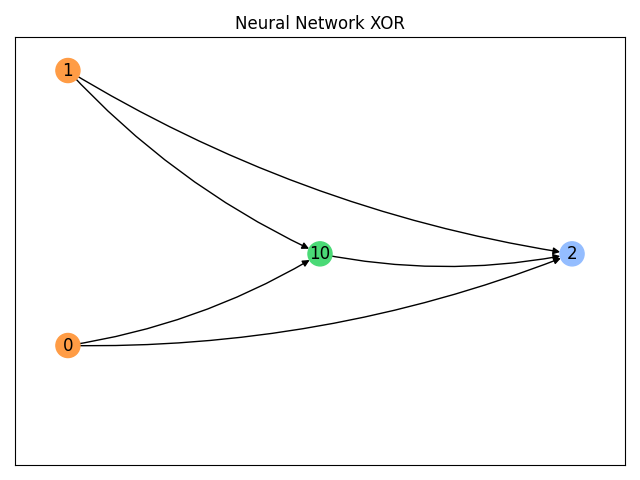
\includegraphics[width=1.0\textwidth]{./img/xor_single_core/xor_neural_network.png} 
		%\caption{Lösung für das XOR-Problem mit einem \emph{Hidden}-Neuron}
		%\label{fig:xor_solution_minimal}
	\end{minipage}
	\hfill
	\begin{minipage}[b]{0.49\textwidth}
		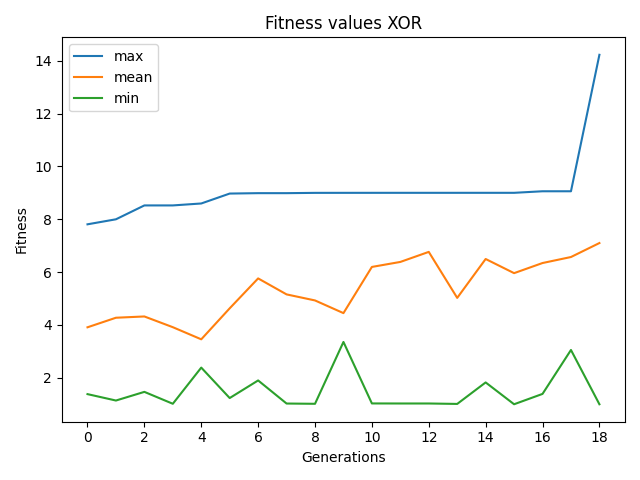
\includegraphics[width=1.0\textwidth]{./img/xor_single_core/xor_fitness_.png} 
		%\caption{Lösung für das XOR-Problem mit einem \emph{Hidden}-Neuron}
	\end{minipage}
	\caption{Links die Lösung für das XOR-Problem mit einem \emph{Hidden}-Neuron, rechts die dazugehörigen Fitnesswerte pro Generation}
	\label{fig:xor_solution_minimal}
\end{figure}
\\\\
Zuletzt soll die tatsächlich erhaltene Lösung genauer betrachtet werden. Im Schnitt hat \ac{NEAT} Lösungen mit 2 oder 3 \emph{Hidden}-Neuronen entwickelt. Allerdings sind auch einige \ac{KNN} entstanden, welche hiervon nur eines und somit die minimale Struktur besitzen, welche zum Lösen des XOR-Problems benötigt wird. Eine solches \ac{KNN}, welches am Ende einer Evaluation entstanden ist, ist in Abbildung \ref{fig:xor_solution_minimal} links dargestellt. Die eigentliche Darstellung ist mithilfe der implementierten Visualisierung  erstellt worden, welche die Pakete NetworkX und Matplotlib nutzt. Bei solchen Darstellungen ist zu beachten, dass die Organgen Neuronen vom Typ \emph{Input}, die grünen vom Typ \emph{Hidden} und die blauen vom Typ \emph{Output} sind. Die Zahlen auf den Neuronen repräsentieren die jeweilige ID während die Pfeile die Verbindungen zwischen den Neuronen darstellen. Für eine bessere Übersichtlichkeit wird in der Darstellung auf die Gewichte verzichtet. Prinzipiell kann eine solche Darstellung auch gestrichelte Verbindungen enthalten. Diese sind dann im Genom deaktiviert und werden nicht für die Berechnungen verwendet. Rechts in der Abbildung ist der Verlauf des maximalen, minimalen und durchschnittlichen Fitnesswertes für jede Generation dargestellt. Auch diese Abbildung wird mit Matplotlib im Rahmen des implementierten \emph{FitnessReporters} automatisch erstellt und zeigt einige interessante Eigenschaften. Der durchschnittliche Fitnesswert steigt trotz einiger Einbrüche relativ kontinuierlich an. Hieraus lässt sich schließen, dass auch die Population im ganzen Fortschritte erzielt. Der maximale Fitnesswert hingegen, stagniert für einige Generationen am Wert $9$. Der Grund hierfür liegt in der Fitnessfunktion. Ein einfaches \ac{KNN} ohne \emph{Hidden}-Neuronen kann drei Werte des XOR-Problems richtig bestimmen. Ist dies der Fall, ergibt die Fitnessfunktion den Wert $9$. Ab diesem Zeitpunkt wird kein Fortschritt des Fitnesswertes erzielt, bis das neue Neuron erfolgreich in die Struktur integriert ist. Der minimale Fitnesswert ist im gesamten Verlauf sehr gering. Der Grund hierfür ist, dass durch unpassende Mutationen oder Rekombinationen Genome entstehen können, bei denen die negativen Eigenschaften überwiegen. 
\begin{figure}[!h]
	\centering
	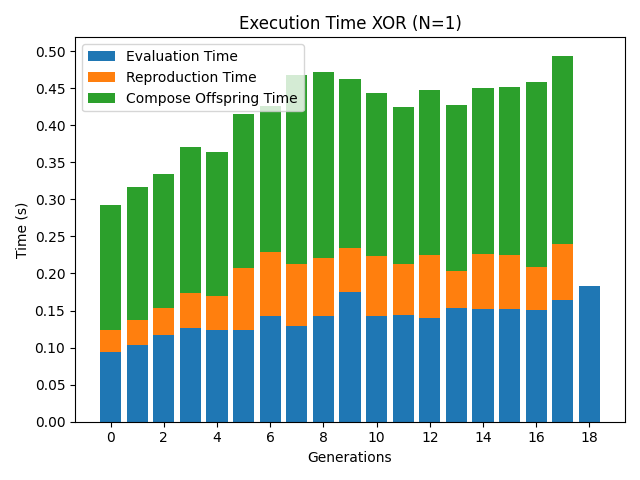
\includegraphics[width=0.5\textwidth]{./img/xor_single_core/xor_time.png} 
	\caption{Ausführungszeiten des XOR-Problems auf einem Raspberry Pi 4 mit einem Prozess}
	\label{fig:xor_single_core_performance}
	% TODO Eventuell Pfeile bei reduce hinzufügen?
\end{figure}
\\\\
Abbildung \ref{fig:xor_single_core_performance} zeigt die Ausführungszeit des Verfahrens in Sekunden für jede Generation an. Auch dieser Graph wird wie die anderen zuvor automatisch mit dem Paket Matplotlib generiert und zeigt drei verschiedene Phasen an. Der blaue Bereich zeigt \emph{Evaluation Time } an, welche die benötigte Evaluationszeit für alle Agenten darstellt. Der grüne Balken repräsentiert die \emph{Compose Offspring Time}, welche die Zeit für die Rekombination und Mutation aller Agenten umfasst. Die verbleibenden Aktionen bezüglich \ac{NEAT}, wie zum Beispiel das Sortieren der Agenten in die verschiedenen Spezies wird im Rahmen der \emph{Reproduction Time} erfasst, welche mit dem grünen Balken repräsentiert wird. Somit wird die Zeit, welche beispielsweise zum Speichern der Zwischenergebnisse benötigt wird nicht erfasst, da diese das Ergebnis verfälschen würde. Insgesamt ist bezüglich des XOR-Problems zu erkennen, dass die Ausführungszeit tendenziell mit zunehmenden Generationen ansteigt. Dies kann durch den erhöhten Rechenaufwand erklärt werden, welcher durch größere \ac{KNN} entsteht. Des weiteren ist auffällig, dass für die letzte Generation keine \emph{Reproduction Time} oder \emph{Compose Offspring Time} erfasst wurde. Der Grund hierfür ist, dass nach der evaluierten Generation die Abbruchbedingung überprüft wird, welche in diesem Fall die Ausführung beendet und daher wird  keine neue Generation erstellt. Zuletzt soll noch die allgemeine Ausführungszeit und das Verhältnis der verschiedenen Phasen betrachtet werden. Zu erkennen ist, dass die Ausführungszeit pro Generation weniger als eine halbe Sekunde benötigt. Dies ist vor allem für Testzwecke ein großer Vorteil, da der Effekt von Änderungen schnell beobachtet werden kann. Zusätzlich ist zu erkennen, dass die meiste Zeit für das Erstellen und Mutieren von neuen Genomen und Agenten benötigt wird. Allerdings ist diese Verteilung unter Umständen nicht repräsentativ, da die XOR-Funktion ein sehr einfaches Problem ist, welches nur wenige Instruktionen umfasst. Daher werden im nächsten Kapitel aufwändigere Optimierungsprobleme betrachtet.

% !TeX spellcheck = de_DE
\section{Optimierungsprobleme}
\label{sec:analysis_optimzation_problems}
Nach erfolgreicher Verifizierung der Funktionalität wird in diesem Kapitel auf verschiedene andere Optimierungsprobleme eingegangen, anhand derer die Analyse durchgeführt werden soll. Grundsätzlich ist bei der Implementierung zu beachten, dass keine zu aufwändigen Optimierungsprobleme verwendet werden, da der Raspberry Pi 4 grundsätzlich nicht so leistungsfähig ist und die benötigte Optimierungszeit sehr hoch sein kann. Daher werden im folgenden hauptsächlich klassische Probleme des bestärkenden Lernens aus dem OpenAI Gym verwendet. Die ausgewählten Umgebungen sind das \emph{Cartpole}, \emph{MountainCar} und das \emph{Pendulum} Problem. Im Folgenden wird auf die entsprechenden Optimierungsprobleme genauer eingegangen und die Implementierung der Fitnessfunktion und Abbruchbedingung kurz vorgestellt. 

\subsection{Cartpole}
Die \emph{Cartpole} Umgebung, auch als \emph{Pole Balancing} bezeichnet, wurde bereits 1983 das erste mal in Quelle \cite{barto1983neuronlike} vorgestellt und ist auch heute noch ein bekanntes Optimierungsproblem, welches in vielen Publikationen verwendet wird. Auch im OpenAI Gym ist dieses Problem entsprechend der Beschreibung aus Quelle \cite{barto1983neuronlike} enthalten und in Abbildung \ref{fig:cartpole_environment} dargestellt. In der Umgebung befinden sich zwei Gegenstände. Das erste ist ein Waagen, welcher von dem Agenten nach links und rechts bewegt werden kann. Hierauf befindet sich ein Balken, welcher am unteren Ende mit dem Waagen verbunden ist. Entsprechend seiner Position, kann dieser nach links oder rechts kippen. Das Ziel für den Agenten ist, durch Steuerung des Wagens den Balken so lange wie möglich senkrecht zu balancieren. Bezüglich der Abbruchbedingung gilt, dass der Agent scheitert wenn der Balken entweder mehr als $15\degree$ auf eine Seite kippt oder wenn der Wagen sich zu weit vom Zentrum entfernt hat. Als Eingabewerte für das \ac{KNN} werden von der Umgebung vier Werte zur Verfügung gestellt, für welche je ein Eingabeneuron erstellt wird. Dies ist unter anderem die Position und Geschwindigkeit des Wagens, der aktuelle Winkel des Balkens und dessen Änderungsrate. Zusätzlich besitzt das erstellte \ac{KNN} zwei Ausgabeneuronen, welche die jeweilige Richtung repräsentieren. Ist der Aktivierungsgrad des erstens \emph{Output}-Neurons höher als der des zweiten, wird der Wagen nach links bewegt und andernfalls nach rechts.
\begin{figure}[!h]
	\centering
	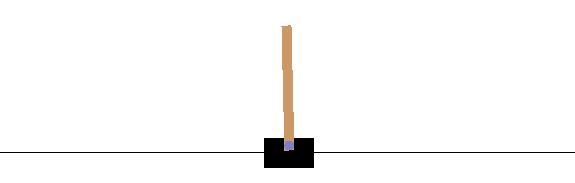
\includegraphics[width=0.5\textwidth]{./img/cartpole_env.JPG} 
	\caption{Darstellung der \emph{Cartpole} Umgebung}
	\label{fig:cartpole_environment}
\end{figure} 
Bevor die Evaluation mit dieser Umgebung durchgeführt wird, müssen noch die Fitnessfunktion, Lösungsbedingung und Konfiguration festgelegt werden. Beim klassischen bestärkenden Lernen, wie es in Kapitel \ref{subsubsec:reinforcment_learning} beschrieben ist, erhält der Agent nach jedem Zeitschritt einen \emph{reward}. Da das OpenAI Gym primär für diese Art des Lernens konzipiert ist, wird auch hier nach jeder Aktion in der Umgebung ein \emph{reward} zurück gegeben. In diesem Fall erhält ein Agent bis er scheitert für jeden Zeitschritt einen \emph{reward} mit der Wertigkeit $1$. Mit diesen muss für neuroevolutionäre Algorithmen eine Fitnessfunktion definiert werden. In diesem Beispiel ist das Vorgehen einfach. Der Fitnesswert wird berechnet indem die erhaltenen \emph{rewards} aggregiert und der erhaltene Wert am Ende der Evaluation quadriert wird. Somit soll wie zuvor beim XOR-Problem besseren Agenten ein proportional höherer Fitnesswert zugewiesen werden. Das Optimierungsverfahren wird abgebrochen, wenn ein Agent den Balken für mindestens 500 Zeitschritte balancieren kann. Die restlichen Parameter wurden aus dem vorherigen Beispiel übernommen und nicht wieder geändert.
\begin{figure}[!h]
	\centering
	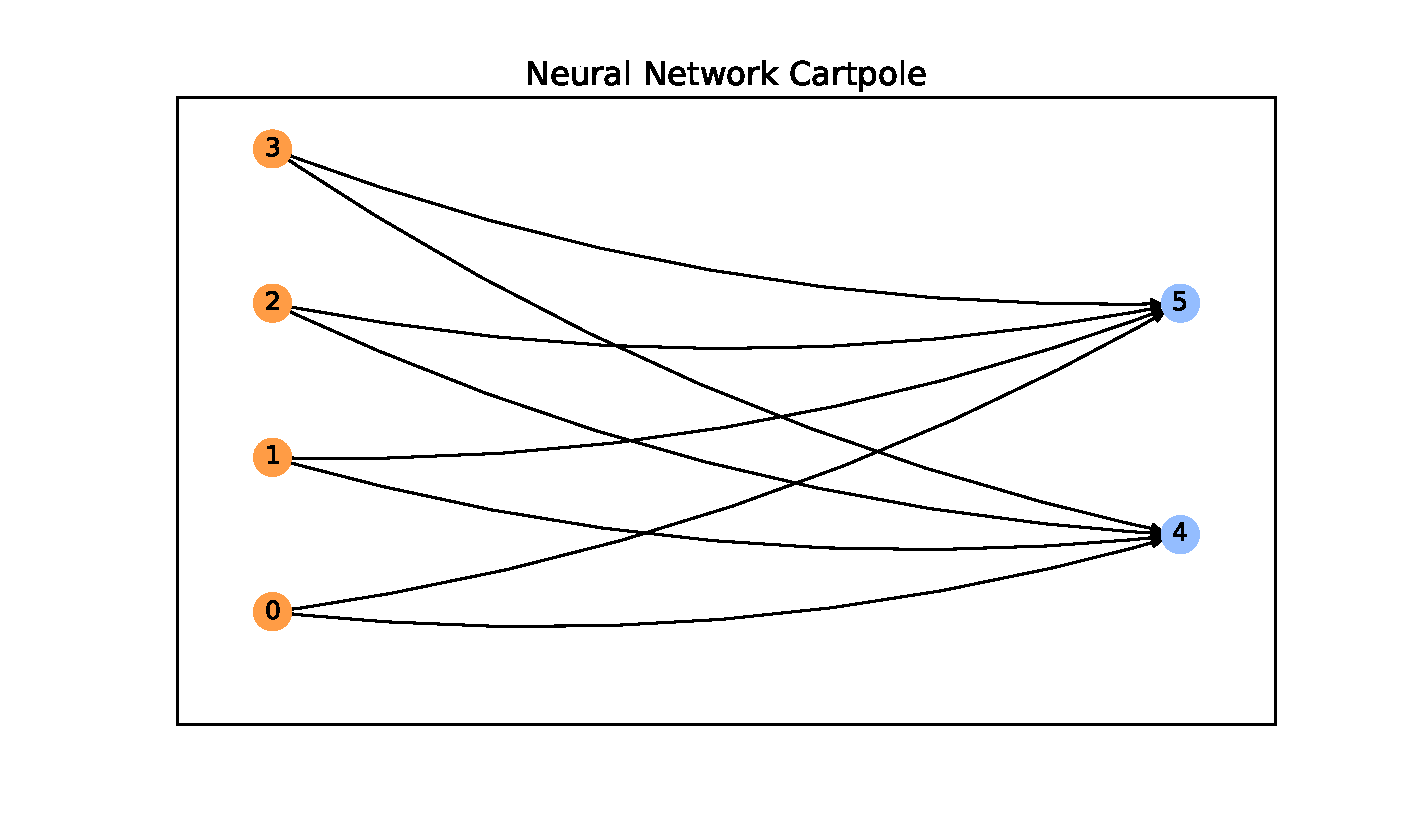
\includegraphics[width=0.7\textwidth]{./img/pole_balancing_single_core/cartpole_neuroal_network.pdf} 
	\caption{Struktur des finalen \ac{KNN} im \emph{Cartpole} Optimierungsproblem}
	\label{fig:cartpole_neural_network}
\end{figure}
\\\\
Allerdings stellt sich beim Ausführen dieses Optimierungsproblems heraus, dass es für die Analyse ungeeignet ist. Bereits in der initialen Population, für welche die Agenten zufällig erstellt werden, sind \ac{KNN} vorhanden, die die Abbruchbedingung erfüllen und das Optimierungsproblem lösen. Ein solches ist in Abbildung \ref{fig:cartpole_neural_network} dargestellt. Wie die anderen \ac{KNN} in der initialen Population, besitzt auch dieses keine \emph{Hidden}-Neuronen und zeigt, dass für das Lösen dieses Optimierungsproblem keine komplexen Entscheidungen notwendig sind. Es ist beispielsweise mit dem Winkel des Balken möglich auf die auszuführende Aktion zu schließen. Neigt sich der Balken nach rechts, bewegt sich der Wagen in diese Richtung und umgekehrt. Dies ist einer der Gründe warum dieses Optimierungsproblem im weiteren Verlauf der Arbeit nicht weiter verwendet wird. Ein weiterer Grund ist, dass durch die Fehlende Optimierung keine Ausführungszeiten über mehrere Generationen gemessen werden können, welche eine notwendige Grundlage für den späteren Vergleich sind.

\subsection{Mountain Car}

\subsection{Pendulum}



% !TeX spellcheck = de_DE
\section{Erkenntnisse}
\label{sec:analysis_results}
Nach Darstellung der Optimierungsprobleme erfolgt eine Zusammenfassung der Ergebnisse in diesem Kapitel. Alle vorgestellten Optimierungsverfahren konnten durch die Schnittstelle der Bibliothek schnell und einfach implementiert werden. Dies trifft sowohl auf individuell erstellte Optimierungsprobleme als auch auf Standardprobleme aus dem \emph{OpenAI Gym} zu. Auch die restlichen Anforderungen aus Kapitel \ref{sec:requirements} sind vollständig implementiert. Der gesamte Ablauf des Algorithmus kann mithilfe eines spezifizierten \emph{Seeds} beeinflusst und wiederholt werden. Die verschiedenen Abbildungen im vorherigen Kapitel zeigen, dass die Testergebnisse der Trainingsverfahren gemessen, visualisiert und gespeichert werden können, sodass ein späterer Vergleich mit der parallelisierten Implementierung möglich ist.
\\\\
Die Funktionalität des Algorithmus, neue Strukturen zu entwickeln und zu optimieren, ist mit dem XOR-Problem bewiesen. Mit derselben Konfiguration werden im Vergleich zur originalen Implementierung ähnliche Ergebnisse gemessen. Durch verschiedene Anpassungen konnten bei nachfolgenden Versuchen sogar bedeutend bessere Ergebnisse erzielt werden. Bei Betrachtung der Ausführungszeit ist in diesem Beispiel die Zeit zum Erstellen und Mutieren von Nachkommen der größte Faktor. Aber da das XOR-Problem insgesamt sehr einfach ist und somit aufwendigere Probleme nicht richtig repräsentiert, finden die Ergebnisse im weiteren Verlauf keine Beachtung.
\\\\
Im nächsten Schritt wurden daher die \emph{CartPole}, \emph{MountainCar} und \emph{Pendulum} Umgebung des \emph{OpenAI Gyms} implementiert, welche aufwendiger zu lösen sein sollten als das XOR-Problem. Die Tests haben ergeben, dass die erste Umgebung ungeeignet ist, da bereits die zufällig erstellten \ac{KNN} der ersten Generation das Optimierungsproblem lösen können. Dies trifft nicht auf die zwei anderen Umgebungen zu. Im vorgestellten Szenario wurden für die erste Umgebung $105$ Minuten, für die zweite Umgebung $125$ Minuten zur erfolgreichen Optimierung benötigt. Zwar hat \ac{NEAT} beide Probleme erfolgreich gelöst, dennoch werden die Grenzen des Algorithmus aufgezeigt. Vor allem auf dem Raspberry Pi sind die benötigten Optimierungszeiten für verhältnismäßig kleine Probleme sehr hoch. Große Optimierungsprobleme, bei denen die Eingabevektoren aus mehreren tausend Werten bestehen, können aufgrund der begrenzten Rechenleistung nicht oder nur mit sehr hohem Zeitaufwand optimiert werden. Da der Fokus dieser Arbeit auf dem Vergleich zwischen einer sequenziellen und parallelisierten Implementierung liegt, ist dieser Umstand zu vernachlässigen.
\\\\
Bei Betrachtung der Ausführungszeiten ist sowohl für das \emph{MountainCar} und \emph{Pendulum} Problem ersichtlich, dass die Evaluationsphase der größte Faktor ist. In der ersten Umgebung werden $98\%$, in der zweiten $91\%$ der Ausführungszeit für das Erstellen und Evaluieren der \ac{KNN} verwendet. Da im Falle einer erfolgreichen Parallelisierung in dieser Phase die meiste Ausführungszeit eingespart werden kann, liegt der Fokus im folgenden Kapitel primär darauf. Für die eigentliche Parallelisierung ist wichtig, dass nicht nur die Berechnungen des \ac{KNN} optimiert werden. Im Rahmen der \emph{Evaluation Time} wird neben der benötigten Zeit zum Erstellen und Aktivieren eines \ac{KNN} auch die benötigte Zeit zum Simulieren der Umgebung gemessen. Diese kann einen großen Einfluss auf das Gesamtergebnis haben. An zweiter und dritter Stelle der Priorisierung stehen die Parallelisierungen der Funktionen in den Phasen \emph{Compose Offspring Time} und \emph{Reproduction Time}. Beide haben einen bedeutend geringeren Anteil an der gesamten Ausführungszeit und dementsprechend weniger Zeit kann eingespart werden. Ob und wie diese implementiert werden können, wird in den Kapiteln \ref{sec:future_work} erläutert.
\\\\
Zuletzt soll betont werden, dass bei den vorgestellten Optimierungsproblemen keine generelle Lösungsstrategie entwickelt wird. Hierfür müssten verschiedene Startsituationen in der Evaluationsphase getestet werden, indem beispielsweise jeder Agent in $x$ verschiedenen Umgebungen getestet und der mittlere Fitnesswert verwendet wird. Dies würde die Evaluationszeit um den Faktor $x$ erhöhen, was im gegebenen Anwendungsszenario eine Analyse bedeutend aufwendiger gestalten würde. Mit der parallelisierten Version in Kapitel \ref{sec:lunar_lander} kann ein solches Verfahren umgesetzt und ein entsprechendes \ac{KNN} schneller entwickelt werden.


